\documentclass{article}
\usepackage[utf8]{inputenc}
\usepackage[top=1in, bottom=1in, left=1in, right=1in]{geometry}
% \usepackage{indentfirst}
\usepackage{amsmath}
\usepackage{amssymb}
\usepackage{mathtools}
\usepackage{graphicx}
    \DeclareGraphicsExtensions{.png, .jpeg}
\usepackage{caption}

% custom macros
\newcommand*{\doublebar}[1]{\overline{\overline{#1}}}
\newcommand*{\unknown}[0]{\;?\;}
\DeclareMathOperator*{\argmax}{argmax}


% main document
\title{MATH 786: Cooperative Game Theory \\ HW04}
\author{Terence Henriod}
\date{\today}

\begin{document}

\maketitle

\begin{abstract}
Assignment games, permutation games, partially ordered sets, lattices.
\end{abstract}


\newpage
\begin{enumerate}
\item Let $N = \{1, \dots, N\}$ be the set of players in a game, and let $K = 2^{N}$. Define the relation $\preceq$ on $K$ by: $S \preceq T$ if and only if $S$ is a subset of $T$.
    \begin{enumerate}
    \item Verify that $K$ is a poset under the relation $\preceq$. \\

    \textit{Solution}: \\
    In order for $K$ to be a poset under $\preceq$, it must satisfy the properties of reflexivity, anti-symmetry, and transitivity.

        \begin{itemize}
        \item Reflexivity: $x \preceq x$ for all $x \in K$ \\
        Any set is a subset of itself (although not a \emph{proper} subset), so this is true for $K$.

        \item Anti-symmetry: $x \preceq y \text{ and } y \preceq x \implies x = y$ for all $x, y \in K$ \\
        If two sets are subsets of each other, then they must contain precisely the same elements and therefore be the same set. This is true for $K$.

        \item Transitivity: $x \preceq y \text{ and } y \preceq z \implies x \preceq z$ for all $x, y, z \in K$ \\
        If a set is a subset of a set which is the subset of a third set, then the first set must be a subset of the third. This is true for $K$.
        \end{itemize}

    %
    \item What do the join and meet operations turn out to be? \\

    \textit{Solution}: \\
    The join operation is the union of two sets, the meet operation is the intersection of two sets. \\

    %
    \item Is $K$ a lattice under the relation $\preceq$? Justify your answer. \\

    \textit{Solution}: \\
    $K$ is a lattice under $\preceq$. For a set to be a lattice, the join and meet must exist for every pair of elements in $K$; the union and intersection of two sets always exists. \\

    %
    \item State the greatest and least elements of $K$. \\

    \textit{Solution}: \\
    The greatest element of $K$ is $N$; the least element is $\emptyset$. \\

    %
    \end{enumerate}
%
\newpage
\item Give an example of a three-player permutation game which is not an assignment game (you will have to make an argument as to why your permutation game is not an assignment game). \\

\textit{Solution}: \\
\[
C = \begin{pmatrix}
    0 & 1 & 0 \\
    0 & 0 & 1 \\
    1 & 0 & 0 \\
\end{pmatrix}
\]
For a permutation game to be an assignment game, $\Pi$ must map from $N \rightarrow N$ in such a way that a partition of $N$, ($N_{1}, N_{2}$), is produced such that $N_{1} \cap N_{2} = \emptyset$. In this partitioning, any coalition $S$ with $|S| \ge 2$ must not have value if $S \subseteq N_{1}$ or if $S \subseteq N_{1}$. 

In this game, there is no way to partition the players into two such sets. The characteristic function of this game is: \\

\begin{tabular}{| c | c | c |}
\hline
$S$                  & $\Pi^{*}(S)$                                        & $V(S)$          \\
\hline\hline
$\emptyset$          & $\emptyset$                                         & $0$             \\
\hline
$\overline{1}$       & $1 \rightarrow 1$                                   & $0$             \\
\hline
$\overline{2}$       & $2 \rightarrow 2$                                   & $0$             \\
\hline
$\overline{3}$       & $3 \rightarrow 3$                                   & $0$             \\
\hline
$\overline{1, 2}$    & $1 \rightarrow 2, 2 \rightarrow 1$                  & $1 + 0 = 1$     \\
\hline
$\overline{1, 3}$    & $1 \rightarrow 3, 3 \rightarrow 1$                  & $0 + 1 = 1$     \\
\hline
$\overline{2, 3}$    & $2 \rightarrow 3, 3 \rightarrow 2$                  & $1 + 0 = 1$     \\
\hline
$\overline{1, 2, 3}$ & $1 \rightarrow 2, 2 \rightarrow 3, 3 \rightarrow 1$ & $1 + 1 + 1 = 3$ \\
\hline
\end{tabular} \\

All pair coalitions of players in this permutation have value, thus there is no way to partition $N$ as described, so this game cannot be an assignment game.

Intuitively, this game cannot be an assignment game because every player has incentive to buy a house that is not their own (to use the housing market metaphor), but also has a house of relative value to another player, thus each player has both buyer and seller roles to play. If it were an assignment game, there would be at least one player with no incentive to buy anyone else's home, negating their role as a buyer (making them a seller only) and the remaining players must be strictly buyers; the converse would also be true. \\

%
\item Suppose $(N, C)$ is any permutation game. Let $P$ be the set of equilibrium price vectors of this game. Define the relation $\preceq$ on $P$ by: $p^{1} \preceq p^{2}$ if and only if $p^{1}_{i} \le p^{2}_{i}$ for $i = 1, \dots, n$. Is $P$ a lattice under this relation? Give an argument in favor, or else a counter-example. \\

\textit{Solution}: \\
$P$ is a lattice under $\preceq$. Start by recalling that the core of a permutation game is a lattice under the same relation. Then recall that the set of competitive solutions coincides with the core, and therefore must also be a lattice under the same relation. Finally, consider that the set of competitive solutions is directly determined by the set of price vectors due to their linear relationship (so those sets have the same shape), so the set of price vectors must have the same shape, and is therefore also a lattice under $\preceq$.

%
\newpage
\item Give the characteristic function of, and then graph the core of the three-player permutation game defined by:
\[
C = \begin{pmatrix}
 6 &  4 &  1 \\
 9 & 10 &  8 \\
 8 &  5 &  0
\end{pmatrix}
\]

\textit{Solution}: \\\\
\begin{tabular}{| c | c | c |}
\hline
$S$                  & $\Pi(S)$                                            & $V(S)$           \\
\hline\hline
$\emptyset$          & $\emptyset$                                         & $0$              \\
\hline
$\overline{1}$       & $1 \rightarrow 1$                                   & $6$              \\
\hline
$\overline{2}$       & $2 \rightarrow 2$                                   & $10$             \\
\hline
$\overline{3}$       & $3 \rightarrow 3$                                   & $0$              \\
\hline
$\overline{1, 2}$    & $1 \rightarrow 1, 2 \rightarrow 2$                  & $6 + 10 = 16$    \\
\hline
$\overline{1, 3}$    & $1 \rightarrow 3, 3 \rightarrow 1$                  & $8 + 1 = 9$      \\
\hline
$\overline{2, 3}$    & $2 \rightarrow 3, 3 \rightarrow 2$                  & $8 + 5 = 13$     \\
\hline
$\overline{1, 2, 3}$ & $1 \rightarrow 2, 2 \rightarrow 3, 3 \rightarrow 1$ & $4 + 8 + 8 = 20$ \\
\hline
\end{tabular}

\begin{figure}[h!]
  \centering
  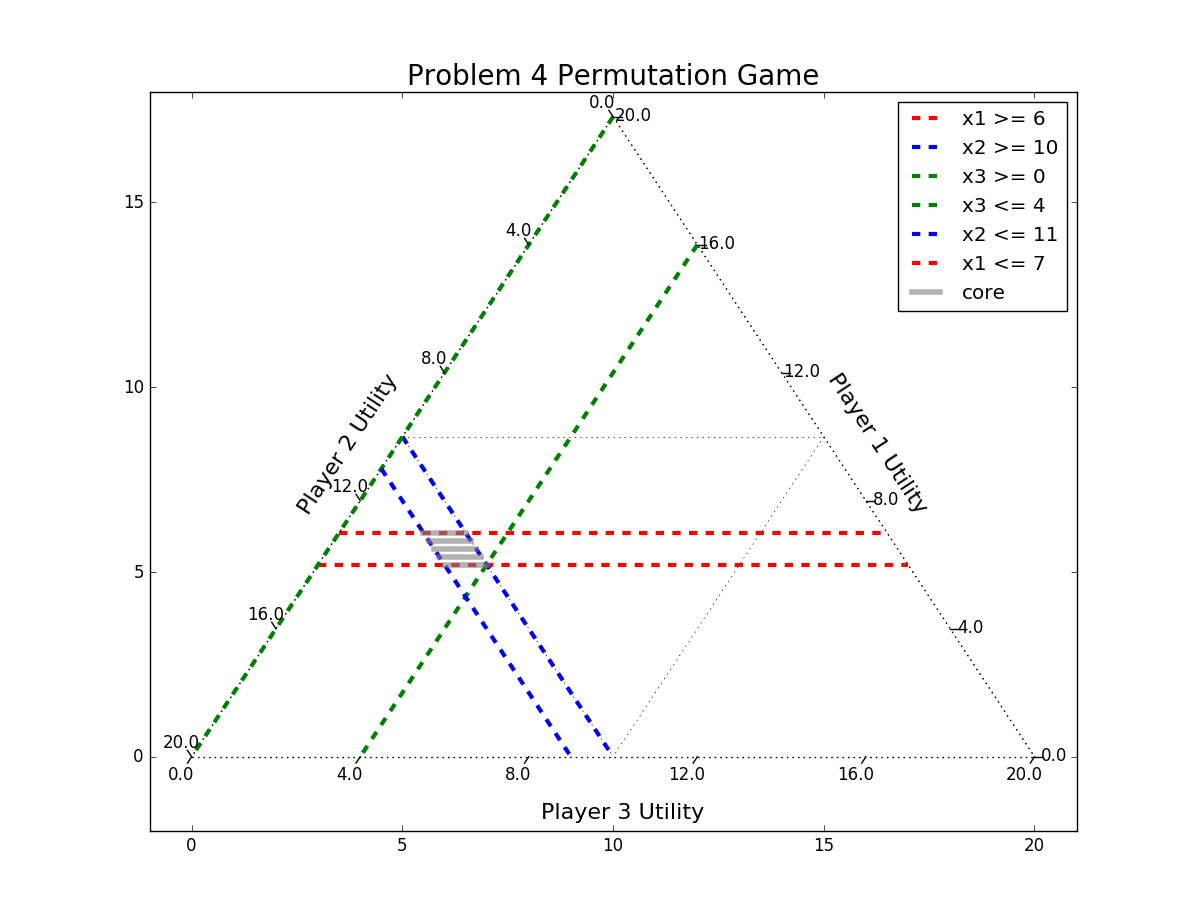
\includegraphics[width=.6\linewidth]{04-04}
  \caption{A graph of the core of the game on the 3-D simplex.}
  \label{fig:04}
\end{figure}
%
% Python code to generate graph
%
% import ternary
% from matplotlib.font_manager import FontProperties
%
% FONT_SIZE = 20
% LINE_ARGS = {'linewidth': 3.0, 'linestyle': '--',}
% CORE_ARGS = {'linewidth': 4.0, 'linestyle': 'solid', 'color': (0.5, 0.5, 0.5, 0.6)}
%
% scale = 20
% figure, tax = ternary.figure(scale=scale)
%
% figure.patch.set_facecolor('white')
%
% # Draw Boundary and Gridlines
% tax.boundary(linewidth=1.0, linestyle=':')
% tax.gridlines(color="black", multiple=scale / 2)
%
% # Set Axis labels and Title
% tax.set_title("Problem 4 Permutation Game", fontsize=FONT_SIZE)
% tax.left_axis_label('Player 2 Utility', fontsize=16)
% tax.right_axis_label('Player 1 Utility', fontsize=16)
% tax.bottom_axis_label('Player 3 Utility', fontsize=16)
%
% # Constraint lines
% tax.left_parallel_line(6, label='x1 >= 6', color='red', **LINE_ARGS)   # x1
% tax.horizontal_line(10, label='x2 >= 10', color='blue', **LINE_ARGS)      # x2
% tax.right_parallel_line(0, label='x3 >= 0', color='green', **LINE_ARGS)  # x3
% tax.right_parallel_line(4, label='x3 <= 4', color='green',  **LINE_ARGS)
% tax.horizontal_line(11, label='x2 <= 11', color='blue', **LINE_ARGS)
% tax.left_parallel_line(7, label='x1 <= 7', color='red', **LINE_ARGS)
%
% # some solid lines to 'fill' the core
% tax.line(
%     # x3, x1, x2
%     (2, 7, 11),
%     (3, 7, 11),
%     **CORE_ARGS,
%     label='core'
% )
% tax.line(
%     (2.25, 6.75, 11),
%     (3.25, 6.75, 11),
%     **CORE_ARGS
% )
% tax.line(
%     (2.5, 6.5, 11),
%     (3.5, 6.5, 11),
%     **CORE_ARGS
% )
% tax.line(
%     (2.75, 6.25, 11),
%     (3.75, 6.25, 11),
%     **CORE_ARGS
% )
% tax.line(
%     (3, 6, 11),
%     (4, 6, 11),
%     **CORE_ARGS
% )
%
% tax.ticks(axis='lbr', multiple=4.0, linewidth=1.0)
%
% # font_prop = FontProperties()
% # font_prop.set_size('small')
% tax.legend()
%
% tax.show()
%

%
\newpage
\item Suppose that one is given an assignment game $C$, with $n$ sellers and $n$ buyers. Without loss of generality, suppose a maximal matching is for seller $j$ to be matched with buyer $j$, $j = 1, \dots, n$. Now suppose further that there is ANOTHER maximal matching, in which seller $j$ is matched with buyer $j + 1$, $j = 1, \dots, n - 1$,  and seller $n$ is matched with buyer $1$. Prove that the core (in terms of the sellers' utilities) is one-dimensional (i.e., is a line). Can you parametrize that line? \\

\textit{Solution}: \\
Consider the efficiency constraints for a vector to be in the core of an assignment game, specifically $u_{i} + v_{\mu^{*}(i)} = c_{i,\mu^{*}(i)}$. A full matching will give $n$ such constraints, so two maximal matchings that are completely different (as in our case) will give $2n$ such constraints. Listing all of the first matching's constraints followed by those of the second matching, we have: \\

\begin{tabular}{r l  c  r l}
$(1)$:  & $u_{1} + v_{1} = c_{1,1}$ &   & $(n + 1)$:  & $u_{1} + v_{2} = c_{1,2}$ \\
$(2)$:  & $u_{2} + v_{2} = c_{2,2}$ &   & $(n + 2)$:  & $u_{2} + v_{3} = c_{2,3}$ \\
$(3)$:  & $u_{3} + v_{3} = c_{3,3}$ &   & $(n + 3)$:  & $u_{3} + v_{4} = c_{3,4}$ \\
        & \dots                     &   &             & \dots                     \\
$(n)$:  & $u_{n} + v_{n} = c_{n,n}$ &   & $(2n)$:     & $u_{n} + v_{1} = c_{n,1}$ \\
\end{tabular} \\

Consider equations $(2)$ and $(n + 1)$, we can solve for $u_{2}$ in terms of $u_{1}$:
\begin{align*}
u_{2} + v_{2} = c_{2,2} &\implies v_{2} = c_{2,2} - u_{2}             &\text{by } (2)   \\
u_{1} + v_{2} = c_{1,2} &\implies u_{1} + c_{2,2} - u_{2} = c_{1, 2}  &\text{substituting for } v_{2} \text{ in } (n + 1) \\
                        &\implies u_{2} = u_{1} + c_{2,2} - c_{1,2}   &\text{rearranging for } u_{2}
\end{align*}

Now that we have $u_{2}$ in terms of $u_{1}$, we can solve for $u_{3}$ in terms of $u_{1}$ as well in a similar manner:
\begin{align*}
u_{3} + v_{3} = c_{3,3} &\implies v_{3} = c_{3,3} - u_{3}             &\text{by } (3)   \\
u_{2} + v_{3} = c_{2,3} &\implies u_{2} + c_{3,3} - u_{3} = c_{2, 3}  &\text{substituting for } v_{3} \text{ in } (n + 2) \\
                        &\implies u_{1} + c_{2,2} - c_{1,2} + c_{3,3} - u_{3} = c_{2,3} &\text{substituting for } u_{2} \text{ in terms of } u_{1} \\
                        &\implies u_{3} = u_{1} + c_{2,2} - c_{1,2} + c_{3,3} - c_{2,3}   &\text{rearranging for } u_{3}
\end{align*}

We can continue in this manner, solving for all of the elements of $\vec{u}$ in terms of $u_{1}$. In general, some element $i$ of $\vec{u}$, other than the first, will have the form:
\[ u_{i} = u_{1} + \sum_{k = 2}^{i}{c_{k,k} - c_{k - 1, k}} \]

Since a core vector (in terms of the sellers' utilities) can be determined by the value only one variable (in our case we chose $u_{1}$), the core must be one-dimensional, i.e., a line. Thus, how we divide payoff between $u_{1}$ and $v_{1}$ determines the payoffs, where the possibilities form a line. The buyers' payoffs can be determined in the same manner, and will also form a line.

The line can be parameterized as $x = \vec{b} + u_{1}\vec{1}$ where $\vec{b}$ and $\vec{1}$ are n-vectors and $\vec{b}$ is a vector such that:

\[ b_{i} = \begin{cases}
  0                                         &\text{ if } i = 1            \\
  \sum_{k = 2}^{i}{c_{k,k} - c_{k - 1, k}}  &\text{ otherwise} 
\end{cases} \]
%
% This is a similar situation to Homework 3 - Problem 3 if $x = 4$.
%

%
\end{enumerate}
%
\end{document}
